% Voor Engelse tekst, gebruik de optie english.
\documentclass[11pt, english]{article}
\usepackage[english]{babel}
\usepackage{listings}
\usepackage{graphicx}
\usepackage[pdfborder={0 0 0}]{hyperref}
\usepackage{caption}
\usepackage{lipsum}
\addtolength{\oddsidemargin}{-1.5cm} 		%linkermarge verkleinen
\addtolength{\textwidth}{3cm}
\addtolength{\topmargin}{-1.5cm}
\addtolength{\textheight}{3.5cm}
\usepackage{chngcntr}
\usepackage[all]{xy}
\usepackage{amsmath}
\usepackage{bbm} 
\usepackage{algpseudocode}
\usepackage{algorithm}
\usepackage{amssymb}  
\usepackage{amsthm}     
\usepackage{enumerate}
\usepackage{url}
\graphicspath{ {./plaatjes/} }
\title{Graphical Model}
\author{Politeness group}
% Wiskunde-omgevingen
%
\newcommand{\field}[1]{\mathbb{#1}}
\newcommand{\R}{\field{R}} % reele getalen
\newcommand{\N}{\field{N}} % natuurlijke getallen
\newcommand{\C}{\field{C}} % complexe getallen
\newcommand{\Z}{\field{Z}} % gehele getallen
\newcommand{\Hom}{\text{Hom}}
\DeclareMathOperator{\im}{Im}
\DeclareMathOperator{\Ker}{Ker}
\usepackage[usenames, pdftex]{color}
\definecolor{OliveGreen}{rgb}{0,0.6,0}
\lstset{
    language=matlab,
    basicstyle=\ttfamily\small,
    commentstyle=\color{OliveGreen}}
\begin{document}
\maketitle
\begin{figure}
    \centering
    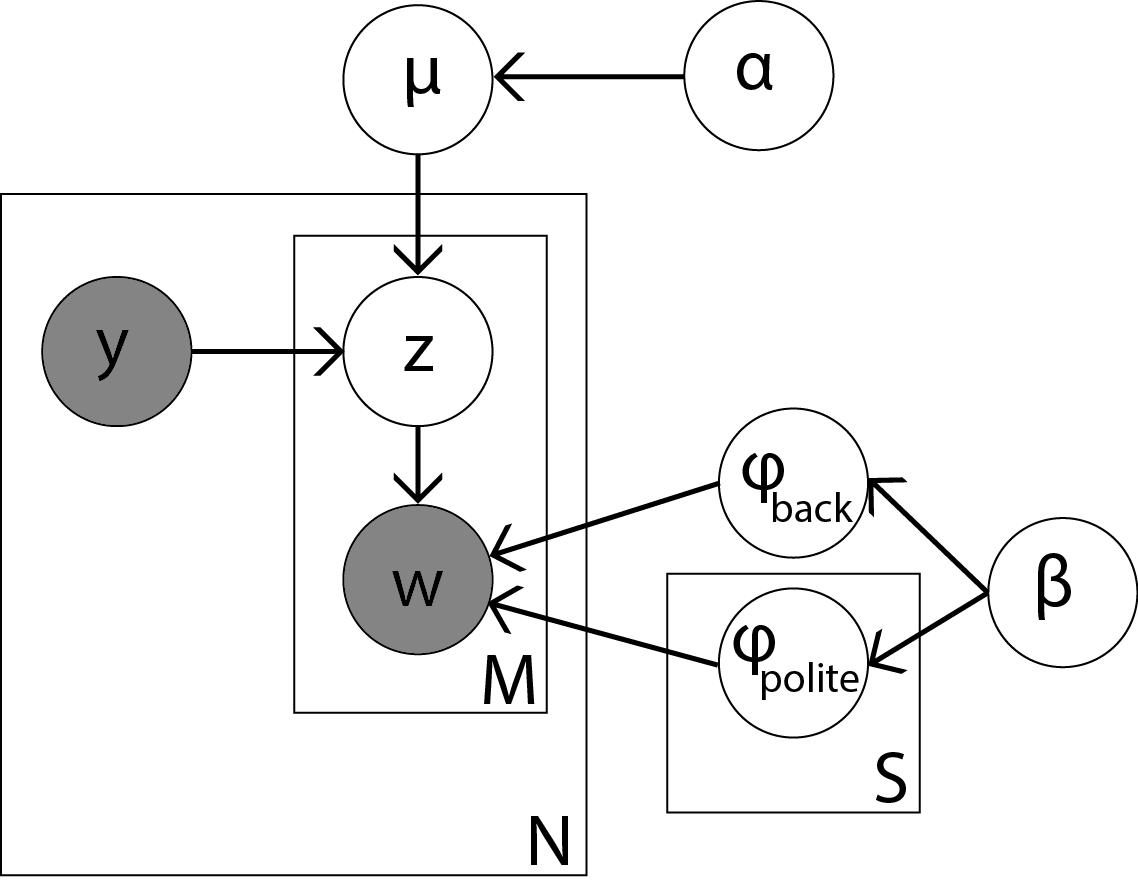
\includegraphics[scale=0.5]{Model}
    \caption{Graphical model for our topic model.}
\end{figure}
Let $N$ sentences be given containing words $w_{n1},\dots,w_{nM_n}$ for $n=1,\dots,N$. Each word $w_{nm}$ is generated from a distribution of words $\phi_z$, with the possibilities background (neutral), polite or impolite. These $\phi_z$ are Dirichlet distributions with hyperparameter $\beta$. In order to see which distribution a word is generated from, we attach a (latent) variable $z_{nm}$ to each word. Furthermore, a sentence as a whole can be either polite or impolite, which we store in the (observed) variable $y_n$. 

We make the assumption that polite sentences only contain words that were generated from the polite distribution or the background distribution, where the distribution over both distributions is specified by $\mu$. Similarly, $\mu$ is used for impolite sentences to give the distribution over impolite words and backgrounds words. The distribution given by $\mu$ is a Beta distributions with hyperparameter $\alpha=(\alpha_1,\alpha_2)$. The generation of a topic $z_{nm}$ for word $w_{nm}$ is sampled from some $\mu$, where $y_n$ picks either the polite or the impolite distribution.

In order to visualize which words are polite, which are impolite and which are background, we want to sample the topics $z_i$ for the words $w_i$ of a new sentence. For this purpose, the sentence first needs to be classified as either polite or impolite (which gives the value for $y$) and then we need to sample from $p(z_{i}|W,y,\Phi,z_{-i},\mu)$, where $W$ consists of all words in the sentence, $z_{-i}$ are the other topics and $\Phi = \phi_1,\phi_2,\phi_3=\phi_{background},\phi_{polite},\phi_{impolite}$. 

We see that
\[
p(Z,W,Y,\mu,\Phi|\alpha,\beta)=p(\mu |\alpha) \prod_{i=1}^3 p(\phi_i|\beta) \prod_{n=1}^N  \prod_{m=1}^M p(w_{nm}|\phi_{z_{nm}})p(z_{nm}|\mu,y_n),
\]
hence
\[
p(Z,W|\alpha,\beta)=\int p(Z,W,Y,\mu,\Phi|\alpha,\beta) d\Phi d\mu =
\]
\[
\left(\int p(\mu |\alpha)\prod_{n=1}^N  \prod_{m=1}^M p(z_{nm}|\mu,y_n)d\mu \right) \left( \int \prod_{i=1}^3 p(\phi_i|\beta) \prod_{n=1}^N  \prod_{m=1}^M p(w_{nm}|\phi_{z_{nm}}) d\Phi \right).
\]
Both parts will be worked out separately. 
\[
\int p(\mu|\alpha)\prod_{n=1}^N  \prod_{m=1}^M p(z_{nm}|\mu, y_n)d\mu=
\]
\[
\int \frac{\Gamma(\alpha_1+\alpha_2)}{\Gamma(\alpha_1)\Gamma(\alpha_2)} \mu^{\alpha_1-1}(1-\mu)^{\alpha_2-1} \prod_{i=1}^2 \prod_{\{n:y_n=i\}}  \prod_{m=1}^{M_n} p(z_{nm}|\mu,y_n)d\mu=
\]
\[
 \frac{\Gamma(\alpha_1+\alpha_2)}{\Gamma(\alpha_1)\Gamma(\alpha_2)} \int  \mu^{\alpha_1-1}(1-\mu)^{\alpha_2-1} \prod_{i=1}^2 \prod_{\{n:y_n=i\}} \mu^{C(0,n)}(1-\mu)^{C(1,n)}d\mu
\]
where $C(0,n),C(1,n)$ denotes the number of background or (im)polite words in sentence $n$ respectively. We rewrite this expression further:
\[
\frac{\Gamma(\alpha_1+\alpha_2)}{\Gamma(\alpha_1)\Gamma(\alpha_2)}
\int  \mu^{\alpha_1-1}(1-\mu)^{\alpha_2-1} \mu^{ \sum_{i=1}^2  \sum_{\{n:y_n=i\}}C(0,n)}(1-\mu)^{\sum_{i=1}^2  \sum_{\{n:y_n=i\}}C(1,n)}d\mu=
\]
\[
 \frac{\Gamma(\alpha_1+\alpha_2)}{\Gamma(\alpha_1)\Gamma(\alpha_2)}
\int  \mu^{\alpha_1-1+C(0)}(1-\mu)^{\alpha_2-1+C(1))}d\mu=
\]
\[
\frac{\Gamma(\alpha_1+\alpha_2)}{\Gamma(\alpha_1)\Gamma(\alpha_2)} \frac{\Gamma(\alpha_1+C(0))\Gamma(\alpha_2+C(1))}{\Gamma(\alpha_1+\alpha_2+C(0)+C(1))}\propto
\frac{\Gamma(\alpha_1+C(0))\Gamma(\alpha_2+C(1))}{\Gamma(\alpha_1+\alpha_2+C(0)+C(1))}
\]
for $C(0)$ the total number of background tags, and $C(1)$ the total number of (im)polite tags.
Before rewriting the second integral, note that we assume a fixed vocabulary of some size $V_i$ of possible words that the $\phi_i$ can generate.
\[
\int \prod_{i=1}^3 p(\phi_i|\beta) \prod_{n=1}^N  \prod_{m=1}^M p(w_{nm}|\phi_{z_{nm}}) d\Phi \propto
\]
\[
\int \prod_{i=1}^3 \prod_{w=1}^{V_i}\phi_i(w)^{\beta-1} \prod_{i=1}^3 \prod_{w=1}^V \phi_i(w)^{C_i(w)} d\Phi=
\]
\[
 \prod_{i=1}^3 \int \prod_{w=1}^{V_i} \phi_i(w)^{\beta-1+C_i(w)} d\phi_i= \prod_{i=1}^3 \frac{\prod_{w=1}^{V_i}\Gamma(\beta+C_i(w))}{\Gamma(\sum_{w=1}^{V_i}\beta+C_i(w))}
\]
for $C_i(w)$ the number of $(n,m)$ such that $w_{nm}=w$ and $z_{nm}=i$.

Combining the equations above gives
\[
p(Z,W,Y,\mu,\Phi|\alpha,\beta)= \prod_{i=1}^3 \frac{\prod_{w=1}^{V_i}\Gamma(\beta+C_i(w))}{\Gamma(\sum_{w=1}^{V_i}\beta+C_i(w))}\times \frac{\Gamma(\alpha_1+C(0))\Gamma(\alpha_2+C(1))}{\Gamma(\alpha_1+\alpha_2+C(0)+C(1))}
\]
such that 
\[
p(z_{nm}=i|Z_{-nm}, W_{-nm}, \Phi,\mu)= \frac{p(z_{nm}=i,Z_{-nm},W,Y,\mu,\Phi|\alpha,\beta)}{p(Z_{-nm},W_{-nm},Y,\mu,\Phi|\alpha,\beta)}\propto
\]
\[
\frac{\Gamma(\alpha_1+C(0))\Gamma(\alpha_2+C(1))\Gamma(\alpha_1+\alpha_2+C(0)+C(1)-1)}{\Gamma(\alpha_1+\alpha_2+C(0)+C(1))\Gamma(\alpha_1+C(0)-\delta_{i,\text{back}})\Gamma(\alpha_2+C(1)-\delta_{i,\text{(im)polite}})} \times
\]
\[
\frac{\Gamma(\beta+C_i(w_{nm}))][\Gamma(\sum_{w=1}^{V_i}\beta+C_i(w)-\delta_{w,w_{nm}}]}{[\Gamma(\sum_{w=1}^{V_i}\beta+C_i(w))][\Gamma(\beta+C_i(w_{nm})-1]}.
\]
The equality $x-1=\frac{\Gamma(x)}{\Gamma(x-1)}$ and some simplifications give
\[
\frac{\Gamma(\alpha_\delta+C(\delta)-1)}{\alpha_1+\alpha_2+C(0)+C(1)-1}
\times \frac{\beta+C_i(w_{nm})-1}{-1+V_i\beta + \sum_{w=1}^{V_i} C_i(w)}
\]
for $\delta = \delta_{i,\text{(im)polite}}$, $V_i$ the number of words in the vocubulary of $\phi_i$, $C(0),C(1)$ the number of background respectively (im)polite words and $C_i(w) = \#\{(a,b):w_{ab}=w$ and $z_{ab}=i\}$.
\end{document}